% !TeX program = xelatex
% Báo cáo ngắn gọn: 5 phương pháp + kiến trúc suy luận M2 + demo custom_suite + hạn chế + kế hoạch.
% Biên dịch: xelatex -interaction=nonstopmode "[17 - 10] - Báo cáo.tex"
% Số liệu: results/*/metrics.json + threshold.json, ngưỡng chọn trên validation.
% Hình kiến trúc M2: images/Pipeline.png (tạo từ prompt reports/figures/m2_pipeline_prompt.md;
% số liệu trong ảnh khớp bản M2-512: max_length 512, ngưỡng 0,66, P(clone) 1,000).
\documentclass[11pt,a4paper]{article}

\usepackage{fontspec}
\setmainfont{Times New Roman}
\usepackage[a4paper,top=2.0cm,bottom=2.0cm,left=2.2cm,right=1.9cm]{geometry}
\usepackage{booktabs}
\usepackage{graphicx}
\usepackage{enumitem}
\usepackage[vietnamese]{babel}
\usepackage{xcolor}
\usepackage{float}
\definecolor{evyellow}{HTML}{B8860B}
\newcommand{\mline}[1]{#1}
\newcommand{\eline}[1]{\colorbox{evyellow!30}{#1}}
% Màu cặp tương ứng: hai phía cùng số là hai đoạn model cho là khớp nhau.
% Màu xoay vòng theo số cặp, cặp 8 trùng màu cặp 0.
\definecolor{pc0}{HTML}{F4B6C2}
\definecolor{pc1}{HTML}{B5D8F7}
\definecolor{pc2}{HTML}{B8E6B8}
\definecolor{pc3}{HTML}{F7E08B}
\definecolor{pc4}{HTML}{D9C2F0}
\definecolor{pc5}{HTML}{F5C99B}
\definecolor{pc6}{HTML}{A8E0E0}
\definecolor{pc7}{HTML}{E8C39E}
\newcommand{\pline}[2]{%
  \ifcase#1\colorbox{pc0}{#2}\or\colorbox{pc1}{#2}\or\colorbox{pc2}{#2}\or%
  \colorbox{pc3}{#2}\or\colorbox{pc4}{#2}\or\colorbox{pc5}{#2}\or%
  \colorbox{pc6}{#2}\or\colorbox{pc7}{#2}\fi}

\title{\vspace{-1.0cm}\textbf{Báo cáo kết quả huấn luyện \& Thử nghiệm}\\[4pt]
       {\normalsize Đề tài: Phát hiện trùng lặp mã nguồn C/C++ và Python}}
\date{\today}

\begin{document}
\maketitle
\vspace{-0.8cm}
\section{Kết quả tuần này}
\begin{itemize}[leftmargin=*,itemsep=0pt,topsep=2pt,parsep=0pt]
\item Tạo bộ test thay đổi vòng lặp \texttt{for}/\texttt{while}/\texttt{do-while},
  đổi IO và tên biến, thêm cặp non-clone khó.
\item 12-10: chạy thêm M1-512, M2-512 (warm-start từ checkpoint 256, \texttt{max\_length} 512, 2 epoch).
\item 15-10: chạy thêm M5-512 (Hybrid trên nền encoder 512, 2 epoch).
\item 17-10: chuyển demo và mục minh hoạ sang bản 512 cho M1/M2/M5 (ngưỡng lấy theo
  \texttt{threshold.json} của run 512), chấm lại bộ test \texttt{custom\_suite}.
\end{itemize}

\section{Kết quả huấn luyện}
F1 trên tập val theo từng epoch, ngưỡng chọn bằng val.\\[2pt]
{\small
\centering
\setlength{\tabcolsep}{4pt}
\resizebox{\textwidth}{!}{%
\begin{tabular}{lcccccccc}
\toprule
\textbf{Epoch} & \textbf{M3} & \textbf{M4} & \textbf{M1-256} & \textbf{M2-256} & \textbf{M1-512} & \textbf{M2-512} & \textbf{M5-256} & \textbf{M5-512} \\
\midrule
E0  & 0,789 & 0,782 & 0,919 & \textbf{0,915} & \textbf{0,921} & 0,932 & \textbf{0,914} & \textbf{0,915} \\
E1  & 0,814 & 0,773 & \textbf{0,919} & 0,914 & 0,918 & \textbf{0,933} & 0,893 & 0,900 \\
E2  & 0,841 & 0,806 & 0,912 & 0,911 & --- & --- & 0,859 & --- \\
E3  & \textbf{0,853} & 0,794 & --- & --- & --- & --- & 0,879 & --- \\
E4  & 0,804 & 0,833 & --- & --- & --- & --- & --- & --- \\
E5  & 0,823 & 0,816 & --- & --- & --- & --- & --- & --- \\
E6  & 0,841 & 0,804 & --- & --- & --- & --- & --- & --- \\
E7  & --- & 0,817 & --- & --- & --- & --- & --- & --- \\
E8  & --- & 0,816 & --- & --- & --- & --- & --- & --- \\
E9  & --- & 0,836 & --- & --- & --- & --- & --- & --- \\
E10 & --- & 0,827 & --- & --- & --- & --- & --- & --- \\
E11 & --- & 0,830 & --- & --- & --- & --- & --- & --- \\
E12 & --- & 0,837 & --- & --- & --- & --- & --- & --- \\
E13 & --- & 0,838 & --- & --- & --- & --- & --- & --- \\
E14 & --- & \textbf{0,842} & --- & --- & --- & --- & --- & --- \\
\bottomrule
\end{tabular}}\par}
Trong đó: M1 = CodeBERT, M2 = GraphCodeBERT, M3 = ASTNN, M4 = CPG-GNN, M5 = Hybrid.

\section{Kết quả test}
{\small\centering
\resizebox{\textwidth}{!}{%
\begin{tabular}{lccccc}
\toprule
\textbf{PP} & \textbf{Prec.} & \textbf{Rec.} & \textbf{F1} & \textbf{AUC} & \textbf{Ngưỡng} \\
\midrule
M3            & 0,760 & 0,894 & 0,821 & 0,889 & 0,420 \\
M4            & 0,723 & 0,887 & 0,797 & 0,882 & 0,470 \\
M1-256        & 0,931 & 0,890 & 0,910 & 0,973 & 0,590 \\
M2-256        & 0,883 & 0,933 & 0,907 & 0,971 & 0,430 \\
M1-512        & 0,947 & 0,935 & \textbf{0,941} & \textbf{0,987} & 0,210 \\
M2-512        & 0,951 & 0,959 & \textbf{0,955} & \textbf{0,991} & 0,660 \\
M5-256        & 0,905 & 0,922 & \textbf{0,913} & 0,970 & 0,370 \\
M5-512        & 0,961 & 0,942 & \textbf{0,952} & 0,988 & 0,010 \\
\bottomrule
\end{tabular}}\par}

\subsection{So sánh 256 và 512 token}
Lên 512 token thì cả ba đều tăng điểm:
\begin{itemize}[leftmargin=*,itemsep=0pt,topsep=2pt,parsep=0pt]
\item M1: 0,910 $\to$ 0,941.
\item M2: 0,907 $\to$ 0,955.
\item M5: 0,913 $\to$ 0,952.
\end{itemize}

\section{Minh hoạ}
Minh hoạ dùng bộ test \texttt{data/custom\_suite} (26 cặp). M1, M2 và M5 chấm bằng bản
512 — bản đã chốt dùng cho demo và báo cáo; M3 và M4 không có biến thể 512 (một cái làm
việc trên cây AST, một cái trên node CPG) nên giữ nguyên bản gốc.\\[2pt]
Cách đọc hình:
\begin{itemize}[leftmargin=*,itemsep=0pt,topsep=2pt,parsep=0pt]
\item Hai phía cùng màu là hai đoạn mà model cho là khớp nhau.
\item Mỗi model có một bảng màu riêng.
\item CodeBERT, GraphCodeBERT, Hybrid ghép theo từng từ (vector encoder).
\item ASTNN ghép theo câu lệnh (vector RvNN); bỏ các span chiếm hơn 60\% file
  và chỉ giữ statement cùng cấp, không bôi cả hàm.
\item CPG-GNN ghép theo dòng (vector node GAT).
\item MOSS tô đúng vùng khớp mà server Stanford trả về; cặp nào không được
  gắn cờ thì để trắng.
\item Ô \colorbox{evyellow!30}{vàng} lẻ là token model dựa vào để cho điểm
  nhưng không ghép được cặp, phần không tô màu là còn lại.
\end{itemize}

\subsection{Cặp clone khó: P1\_combo}
Cùng bài tính tổng 1..n, nhưng bản B viết lại hết: \texttt{for} đổi thành
\texttt{while}, \texttt{cin/cout} đổi thành \texttt{scanf/printf}, đổi tên biến,
đảo điều kiện, thêm biến thừa.
Cả 5 model đều cho là clone (M1 1,000, M2 1,000, M3 0,812, M4 0,915, M5 1,000), đúng cả.
Riêng MOSS cho 0,000 nên bỏ sót cặp này, do server chỉ trả top match nên mấy cặp
Type-3/4 viết lại nhiều không được gắn cờ.
{\shorthandoff{"}\input{../workspace/demo_suite_P1_combo.tex}
\input{../workspace/demo_suite_moss_P1_combo.tex}}

\subsection{Cặp không clone khó: P3\_nonclone}
Cùng khung đọc mảng bằng \texttt{for} rồi in một số, nhưng một bài tìm
\texttt{max} còn bài kia tính tổng.
M1 (0,000), M2 (0,005) và M5 (0,000) đều dưới ngưỡng nên nói đúng là không clone;
ngược lại M3 (0,852) và M4 (0,973) vượt ngưỡng nên nói sai.
MOSS cho 0,000 nên cũng đúng ở cặp này.
Qua đây thấy mấy model cấu trúc (ASTNN, CPG-GNN) dễ bị khung code giống nhau
đánh lừa hơn mấy model transformer.
{\shorthandoff{"}\input{../workspace/demo_suite_P3_nonclone_sum.tex}
\input{../workspace/demo_suite_moss_P3_nonclone_sum.tex}}

\subsection{Cặp bẫy skeleton: P1\_nonclone\_fact (cả 5 model đều sai)}
Cũng là khung \texttt{for} 1..n rồi in một số, nhưng một bài tính tổng còn bài kia
tính giai thừa.
Lần này cả 5 model đều nói sai là clone: M1 0,999, M2 0,991, M3 0,960, M4 0,971, M5 0,723.
MOSS cho 0,000 nên đúng ở cặp này, nhưng đúng kiểu mù (giống cặp ở mục 4.1) chứ
không phải hiểu code.
Cặp \texttt{p4\_n\_square} (số nguyên tố với số chính phương, cùng khung \texttt{for}
trả lời YES/NO) cũng bị sai y hệt nên không vẽ lại hình.
Chiều ngược lại thì không có cặp nào: không có cặp nào GT là clone mà cả 5 model
lại bảo không clone, cả 16 cặp clone đều bắt đúng.
So với bản 256, việc chuyển M1/M2/M5 sang bản 512 sửa thêm 2 chỗ sai nữa trên bộ
test (M2 và M5 ở cặp non-clone \texttt{P2\_nonclone\_digitsum}: 0,505 $\to$ 0,001 và
0,981 $\to$ 0,000) và không làm hỏng cặp nào.
{\shorthandoff{"}\input{../workspace/demo_suite_P1_nonclone_fact.tex}
\input{../workspace/demo_suite_moss_P1_nonclone_fact.tex}}

\section{Kiến trúc phương pháp chính dự kiến (GraphCodeBERT)}

\begin{figure}[H]
\centering
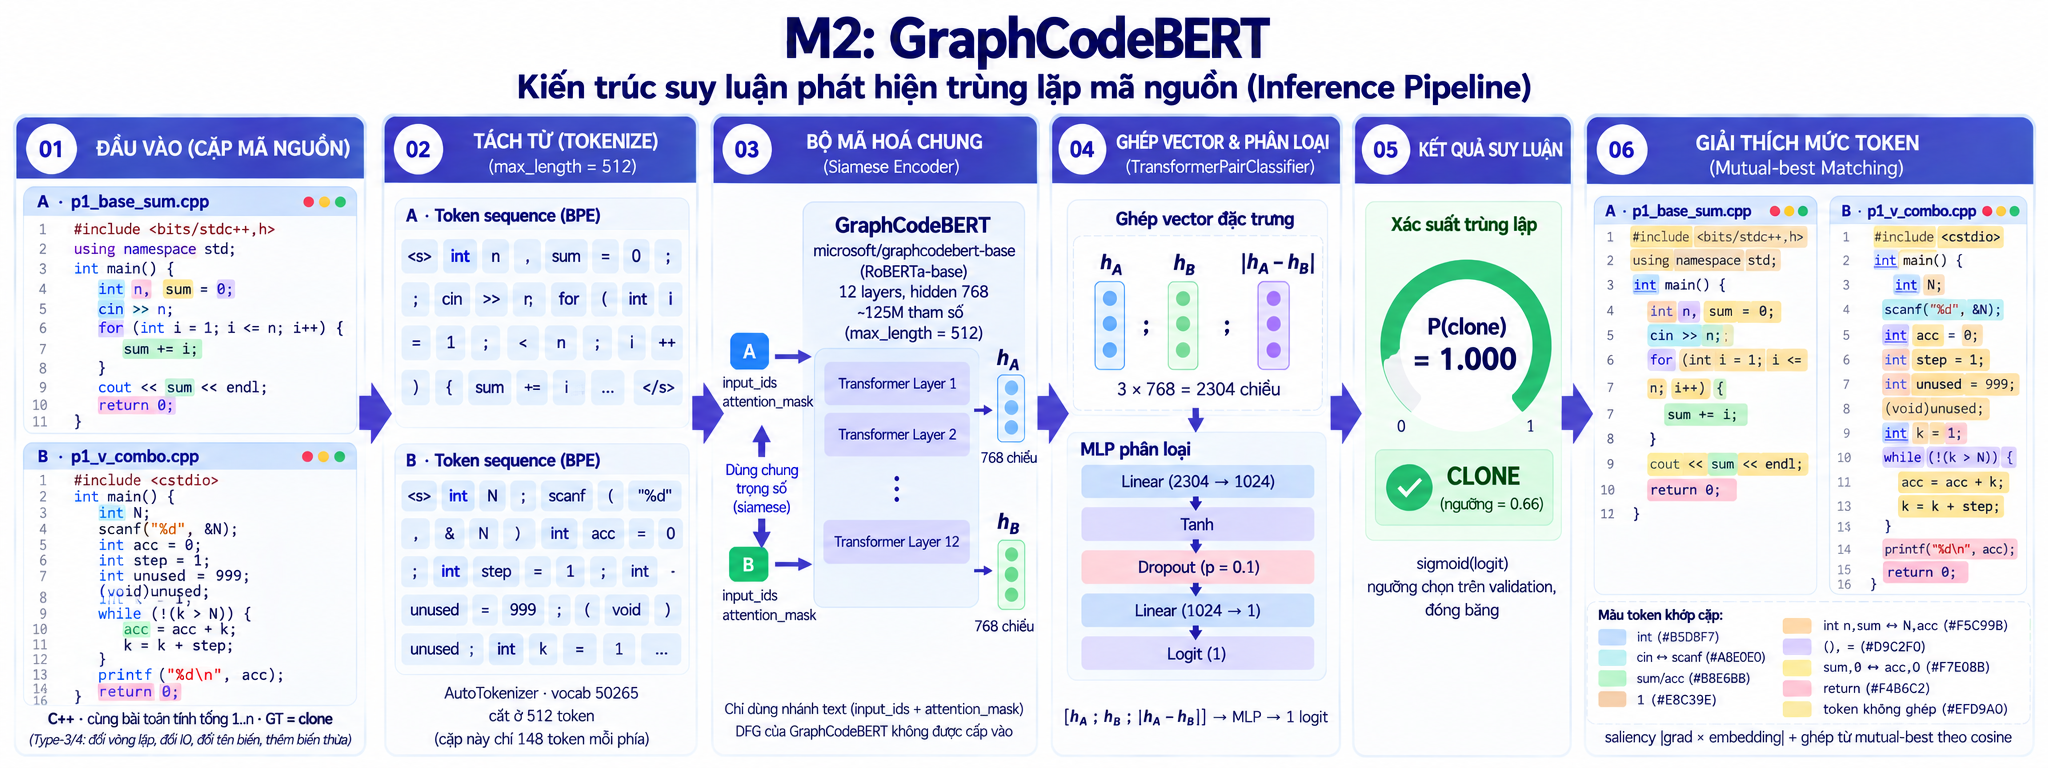
\includegraphics[width=\textwidth]{images/Pipeline.png}
\end{figure}

\section{Hạn chế}
% (để trống — sẽ cập nhật sau)

\section{Kế hoạch tiếp theo}
% (để trống — sẽ cập nhật sau)

\end{document}
